\documentclass[11pt]{article}
\usepackage[margin=0.85in]{geometry}
\usepackage{amsmath,amssymb,booktabs,graphicx,array}
\usepackage[hidelinks]{hyperref}
\usepackage{xurl}
\hypersetup{pdftitle={AFTER: Supplementary material},pdfauthor={Muhammad Usman}}
\DeclareMathSizes{10}{10}{8}{6}
\setlength{\emergencystretch}{2em}
\renewcommand{\thesection}{S\arabic{section}}
\renewcommand{\thetable}{S\arabic{table}}
\renewcommand{\thefigure}{S\arabic{figure}}
\newtheorem{proposition}{Proposition}
\newenvironment{proof}{\par\noindent\textit{Proof.}\ }{\hfill\textit{Q.E.D.}\par}
\title{AFTER: Supplementary Material\\\large Digital Twins for Cyberattack and Recovery Monitoring in Industrial Robots}
\author{Muhammad Usman}
\date{}
\begin{document}
\maketitle
This supplement preserves derivations, earlier experimental detail, complete comparison tables and source-admission records supporting manuscript revision 1.3. All attack/recovery observations are synthetic. The common-input IMU experiment is real-data normal prediction. The newly received voraus-AD file has undergone metadata verification only. No experiment was rerun to produce this revision.

\section{Conditional return bounds}
Let $x_t^0$ denote the uncorrupted same-plant state, $r_t$ its reference, and $y_t=x_t+n_t$ the measurement. For positive training scales, define $\|v\|_s=\max_j|v_j|/s_j$, physical deviation $d_t=\|x_t-x_t^0\|_s$ and observed discrepancy $c_t=\|y_t-r_t\|_s$. The following bounds are conditional geometric arguments, not new interval-observer theory. In particular, the empirical allowance used in the earlier experiment does not establish their assumptions.
\subsection{Conditional error bounds}
\begin{proposition}
If $\|x_t^0-r_t\|_s\le b_t$ and $\|n_t\|_s\le\eta_t$, then
\begin{equation}
 \max(0,c_t-b_t-\eta_t)\le d_t\le c_t+b_t+\eta_t.
 \label{eq:bound}
\end{equation}
\end{proposition}
\begin{proof}
Write $x_t-x_t^0=(y_t-r_t)-n_t-(x_t^0-r_t)$ and apply the triangle and reverse triangle inequalities. Aligned scalar errors attain the extremes, so scalar allowances alone do not generally permit tighter bounds.
\end{proof}

A sufficient return condition at tolerance $\delta$ is $c_t+b_t+\eta_t\le\delta$. This gives a simple feasibility test before any alarm experiment.
\begin{proposition}
Suppose reference and measurement errors lie in coordinate boxes with half-widths $b_{t,j}$ and $\eta_{t,j}$. Return within $\delta$ holds for every pair in those boxes exactly when
\begin{equation}
 \max_j\frac{|y_{t,j}-r_{t,j}|+b_{t,j}+\eta_{t,j}}{s_j}\le\delta.
 \label{eq:box}
\end{equation}
If $b_{t,j}+\eta_{t,j}>\delta s_j$ in any coordinate, no observation can satisfy this condition.
\end{proposition}
\begin{proof}
In each coordinate, the two admissible errors can align against the measured displacement. Their summed magnitude attains the triangle-inequality bound. The observed absolute displacement is nonnegative, yielding the infeasibility statement.
\end{proof}

These statements are conditional geometric facts. The simulated sensors have unbounded Gaussian noise, and the experiment uses an empirical discrepancy allowance rather than a verified deterministic enclosure. Specifically, the tested rule requires $c_t+b\le\delta$, where $b$ is the largest observed normal discrepancy. It is a heuristic motivated by the upper-bound form, not an implementation of a proven safety certificate. Because $b$ contains both model error and noise, interpreting it as pure reference uncertainty would be incorrect. A dwell period cannot restore feasibility when $b>\delta$.



\section{Plant and command specification}\label{sec:simulation}
All observations in the attack and recovery simulations are synthetic. The separate IMU prediction study uses a received public nominal recording and is described independently in Supplement~\ref{app:imu}. The simulated plant is a horizontal two-joint point-mass arm governed by
\begin{equation}
 M(q)\ddot q+C(q,\dot q)+B\dot q=\tau.
\end{equation}
Writing $a=m_2l_1l_2$ and $d=m_2l_2^2$,
\begin{align}
 M(q)&=\begin{bmatrix}(m_1+m_2)l_1^2+d+2a\cos q_2&d+a\cos q_2\\d+a\cos q_2&d\end{bmatrix},\\
 C(q,\dot q)&=a\sin q_2\begin{bmatrix}-2\dot q_1\dot q_2-\dot q_2^2\\\dot q_1^2\end{bmatrix}.
\end{align}
A proportional--derivative (PD) controller requests componentwise saturated torque
\begin{equation}
 \tau^*=\operatorname{clip}\{K_p(q^c-q)+K_d(\dot q^c-\dot q),-20,20\},
\end{equation}
with $K_p=\operatorname{diag}(18,12)$ and $K_d=\operatorname{diag}(4,3)$. Where actuator lag is present, $\dot\tau=(\tau^*-\tau)/T_a$. Nominal masses are $(1,0.8)$ kg, lengths $(0.5,0.4)$ m, and damping coefficients $(0.08,0.06)$. The nominal physics reference retains these parameters; Table~\ref{tab:plants} specifies the actual plants.

\begin{table}[htbp]\centering\small
\caption{Simulated plant configurations. Mass and damping entries multiply the nominal values; noise multiplies the stated sensor standard deviations.}\label{tab:plants}
\setlength{\tabcolsep}{5pt}
\begin{tabular}{lcccrr}\toprule
Plant & Mass factors & Damping factors & Lengths (m) & Lag (s) & Noise\\\midrule
Q1 & (1.10,0.86) & (0.80,1.20) & (0.48,0.42) & 0 & 1.0\\
Q2 & (0.88,1.15) & (1.30,0.85) & (0.53,0.37) & 0.03 & 1.0\\
Q3 & (1.16,1.06) & (0.90,1.40) & (0.46,0.43) & 0.06 & 1.5\\\bottomrule
\end{tabular}
\end{table}

Position and velocity measurements have independent, zero-mean Gaussian noise with standard deviations of 0.0005 rad and 0.002 rad/s before applying the plant multiplier. Each episode contains 1,200 observations at 50 Hz. We integrate with fourth-order Runge--Kutta, using eight substeps per observation, and check a short trajectory with actuator lag against a separate SciPy integration. That check supports numerical consistency. Physical fidelity remains limited: the model excludes gravity, contact, flexibility and thermal effects, and has not been validated against measurements from a real robot.


For phase $\theta(t)$, amplitudes $(a_1,a_2)$ and offset $\phi$, the approved positions are
\begin{align}
q_1^c&=a_1\sin\theta+0.025\sin(2.3\theta),\\
q_2^c&=a_2\sin(\theta+\phi)+0.018\sin(1.7\theta).
\end{align}
Velocities are analytic derivatives under the causal time-warp rate. The final audit uses task N14 with $\theta=0.49t$, amplitudes $(0.28,0.37)$ and phase 0.93; O14 with $\theta=0.43t+0.008t^2$, amplitudes $(0.33,0.31)$ and phase 0.72; and P14 with $\theta=0.94t+0.18\sin(0.31t)$, amplitudes $(0.35,0.38)$ and phase 1.14. Corruption starts at index 347 and ends before 653, except the eight-sample brief offset. Joint-1 offset is 0.11 rad and slowdown rate is 0.72. Authorized changes update the approved path; unauthorized changes do not. The model state does not reset at those indices.

Commissioning uses rates 0.35, 0.7 and 1.1, amplitudes $(0.22+0.04i,0.34-0.025i)$ and phase $0.5+0.3i$ for $i=0,1,2$, covering unchanged, authorized-offset and authorized-slowdown conditions. The earlier 19 normal episodes use rate $0.32+0.047i$, amplitudes $(0.23+0.012(i\bmod7),0.29+0.013(i\bmod9))$ and phase $0.4+0.06(i\bmod11)$. Later studies reuse nine for development, five for calibration and five as archived checks; the archived checks are not new independent data. Source configurations retain every earlier task and condition.

The final interface excludes true states, attack schedules, executed malicious commands and actual plant parameters from inference settings. Earlier E1 code received a broader episode dictionary; source inspection and restricted-input replays support its actual information use, but that interface itself did not enforce isolation. Missing approved-command history makes command-dependent E1 monitors unknown for the rest of an episode. Those observations remain in coverage and missed-event denominators. The final seven-condition audit does not include the missing-context condition.

\section{Earlier results and full final metrics}
\subsection{E1: original recovery comparison}
E1 comprises 216 episodes and 13 methods, with 237,600 eligible points and 135 intervention events. Twenty-seven events have missing command context. Nineteen clean episodes provide 20,900 eligible calibration points; the principal state-machine threshold search allows at most 209 alarmed points on this finite population. This differs from the final audit's point-quantile calibration. The additional constant episode band uses rank 19 of 19 episode maxima; shifted tasks do not establish exchangeability or conformal coverage. Matched-entry ablations preserve their own realized alarm burdens.
\begin{table}[htbp]\centering\small
\caption{E1 attack and recovery outcomes, retained from the saved presentation. Clearance counts condition on detected events with measured return.}
\setlength{\tabcolsep}{3pt}\begin{tabular}{lrrrrr}\toprule
Method & Benign & F1 & Overlap/fresh & Early & Clear/return \\\midrule
Persistence & 878 & 0.057 & 127/127 & 127 & 127/127 \\
ARX one-step & 792 & 0.803 & 108/108 & 108 & 108/108 \\
Following point & 794 & 0.808 & 108/108 & 108 & 108/108 \\
Following hysteresis & 993 & 0.785 & 108/108 & 108 & 108/108 \\
Nominal hysteresis & 789 & 0.713 & 108/108 & 45 & 108/108 \\
Nominal fixed return & 621 & 0.657 & 108/108 & 0 & 108/108 \\
Learned point & 819 & 0.700 & 108/108 & 18 & 108/108 \\
Learned hysteresis & 792 & 0.683 & 108/108 & 0 & 108/108 \\
Learned fixed return & 827 & 0.690 & 108/108 & 0 & 108/108 \\
Uncertainty return & 309 & 0.446 & 108/104 & 0 & 36/108 \\
Episode CP band & 0 & 0.744 & 108/108 & 75 & 108/108 \\
Matched no allowance & 140 & 0.709 & 108/108 & 0 & 108/108 \\
Matched no dwell & 20 & 0.453 & 108/108 & 0 & 36/108 \\
\bottomrule\end{tabular}

\end{table}
\begin{table}[htbp]\centering\small
\caption{E1 additional metrics. Unknown states remain eligible, cannot count as detections, and receive AP score $-1$, below valid nonnegative scores.}
\setlength{\tabcolsep}{3pt}\begin{tabular}{lrrrrrr}\toprule
Method & Precision & Recall & AP & Episodes/h & Missed & Known (\%) \\\midrule
Persistence & 0.203 & 0.033 & 0.130 & 480.8 & 8 & 100.0 \\
ARX one-step & 0.868 & 0.748 & 0.770 & 1426.3 & 27 & 90.0 \\
Following point & 0.878 & 0.747 & 0.770 & 793.9 & 27 & 90.0 \\
Following hysteresis & 0.841 & 0.735 & 0.770 & 99.0 & 27 & 90.0 \\
Nominal hysteresis & 0.706 & 0.719 & 0.587 & 84.8 & 27 & 90.0 \\
Nominal fixed return & 0.656 & 0.658 & 0.587 & 48.5 & 27 & 90.0 \\
Learned point & 0.658 & 0.748 & 0.589 & 1054.5 & 27 & 90.0 \\
Learned hysteresis & 0.628 & 0.747 & 0.589 & 62.6 & 27 & 90.0 \\
Learned fixed return & 0.641 & 0.747 & 0.589 & 115.2 & 27 & 90.0 \\
Uncertainty return & 0.318 & 0.747 & 0.589 & 26.3 & 27 & 90.0 \\
Episode CP band & 0.742 & 0.746 & 0.589 & 0.0 & 27 & 90.0 \\
Matched no allowance & 0.675 & 0.747 & 0.589 & 28.3 & 27 & 90.0 \\
Matched no dwell & 0.325 & 0.747 & 0.589 & 28.3 & 27 & 90.0 \\
\bottomrule\end{tabular}

\end{table}
\subsection{E2: normal commissioning}
The finite grid contains ARX orders 4, 8, 16 and 32 and finite impulse response lengths 16, 32 and 64, each with ridge $10^{-7}$, $10^{-5}$ or $10^{-3}$, on three plants: 63 fits. Fitting and selection precede 81 new normal episodes. The selected orders are 8, 16 and 32 with ridge $10^{-7}$. Table~\ref{tab:normalall} retains distinct prediction roles. Forced-latch probes measure normal clearance feasibility, not post-attack recovery. The hard-plant reductions in empirical allowance do not establish a probabilistic or deterministic error bound.
\begin{table}[htbp]\centering\small
\caption{E2 complete normal-reference comparison. Each row has 29,700 eligible observations and 108 forced-latch probes. Selected reference and selected ARX are identical and appear once.}\label{tab:normalall}
\setlength{\tabcolsep}{4pt}\begin{tabular}{llrrrr}\toprule
Plant & Reference & RMSE & Allowance & Feasible (\%) & Clear/probes \\\midrule
Q1 & ARX(4), free & 0.00948 & 0.0553 & 99.80 & 108/108 \\
Q1 & Selected ARX, free & 0.00934 & 0.0553 & 99.82 & 108/108 \\
Q1 & Selected FIR & 0.01211 & 0.2322 & 0.00 & 0/108 \\
Q1 & ARX(4), one-step & 0.00976 & 0.0649 & 97.92 & 108/108 \\
Q1 & Command as state & 0.09584 & 2.1344 & 0.00 & 0/108 \\
Q2 & ARX(4), free & 0.01020 & 0.1469 & 0.00 & 0/108 \\
Q2 & Selected ARX, free & 0.00972 & 0.0716 & 93.32 & 108/108 \\
Q2 & Selected FIR & 0.01693 & 0.3971 & 0.00 & 0/108 \\
Q2 & ARX(4), one-step & 0.01036 & 0.1211 & 0.00 & 0/108 \\
Q2 & Command as state & 0.10423 & 2.1528 & 0.00 & 0/108 \\
Q3 & ARX(4), free & 0.01586 & 0.1913 & 0.00 & 0/108 \\
Q3 & Selected ARX, free & 0.01439 & 0.1175 & 0.00 & 0/108 \\
Q3 & Selected FIR & 0.02215 & 0.4596 & 0.00 & 0/108 \\
Q3 & ARX(4), one-step & 0.01573 & 0.1807 & 0.00 & 0/108 \\
Q3 & Command as state & 0.11251 & 2.2058 & 0.00 & 0/108 \\
\bottomrule\end{tabular}

\end{table}
\subsection{E5: complete additional metrics and plant strata}
The following tables complement the main paper's complete 17-method audit. Alarm starts per hour use the total eligible duration of wholly benign episodes. Their high frequency for point rules reflects repeated short excursions; the metric should be read alongside occupancy. No unknown-state denominator trimming is applied to this audit. All 189 episodes and 3,213 outcomes are retained.
\begin{table}[htbp]\centering\small
\caption{Final audit: unadjusted point precision/recall, benign occupancy, alarm starts per benign hour and missed events.}
\begin{tabular}{lrrrrr}\toprule
Method & Precision & Recall & Benign (\%) & Starts/h & Misses \\\midrule
base point & 0.6434 & 0.9931 & 0.957 & 1537.4 & 0 \\
base return & 0.4777 & 0.9936 & 7.644 & 1208.1 & 0 \\
base long & 0.4699 & 0.9936 & 8.031 & 1208.1 & 0 \\
base dual & 0.4699 & 0.9936 & 8.031 & 1208.1 & 0 \\
linear point & 0.6421 & 0.9930 & 1.004 & 1618.2 & 0 \\
linear dual & 0.4651 & 0.9934 & 8.415 & 1270.7 & 0 \\
RBF point & 0.6445 & 0.9929 & 0.937 & 1501.0 & 0 \\
RBF return & 0.4811 & 0.9932 & 7.466 & 1191.9 & 0 \\
RBF long & 0.4729 & 0.9932 & 7.870 & 1191.9 & 0 \\
RBF dual & 0.4729 & 0.9932 & 7.870 & 1191.9 & 0 \\
RBF dual, no dwell & 0.6214 & 0.9929 & 1.341 & 1501.0 & 0 \\
following point & 0.8575 & 0.9930 & 0.973 & 1618.2 & 0 \\
following dual & 0.5487 & 0.9934 & 8.569 & 1331.3 & 0 \\
RBF following dual & 0.5486 & 0.9934 & 8.617 & 1317.2 & 0 \\
persistence & 0.1286 & 0.0192 & 0.591 & 274.7 & 41 \\
mean (21) & 0.0385 & 0.0046 & 0.094 & 78.8 & 60 \\
base CUSUM & 0.2665 & 0.9887 & 0.962 & 301.0 & 0 \\
\bottomrule\end{tabular}

\end{table}
\begin{table}[htbp]\centering\small
\caption{Primary base-dual versus RBF-dual comparison by plant. Every plant has 29,700 benign points and 36 attack events.}
\setlength{\tabcolsep}{4pt}\begin{tabular}{lrrrrrr}\toprule
Plant & Base benign & RBF benign & Base gaps & RBF gaps & Base fresh & RBF fresh \\\midrule
Q1 & 2397 & 2522 & 0 & 0 & 36 & 36 \\
Q2 & 2646 & 2532 & 2 & 3 & 29 & 33 \\
Q3 & 2113 & 1958 & 0 & 0 & 36 & 36 \\
\bottomrule\end{tabular}

\end{table}
\clearpage
\section{Separate common-input IMU prediction study}\label{app:imu}
\subsection{Release, chronology and permitted information}
This study compares normal prediction when every model receives the same inputs. Its results are reported separately from the command-aware attack comparison. We use the received author-linked CASPER-1-and-2 provider-v2 nominal file \texttt{IMU\_10Hz.csv}, obtained from the \href{https://www.kaggle.com/datasets/hkayan/industrial-robotic-arm-imu-data-casper-1-and-2}{public provider listing}. Its SHA-256 is\nopagebreak[4]
\begin{center}\small\url{1221df9be80c229969f3f21f820837e68ad28f4ccb3949bf4013f00d6d69d62c}.\end{center}
This file differs from the original CASPER-v3 archive, and its exact correspondence to the original paper's runs remains unresolved. It contains nine channels: X/Y/Z measurements from an accelerometer, gyroscope and magnetometer. We could not resolve the timestamp units or whether they record acquisition or arrival. The filename is therefore insufficient evidence for reporting elapsed time or detection delay.

Training uses numeric rows 219--9184 and development uses rows 9185--12006, indexed from zero. The split precedes a trailing width-20 median filter. Each partition loses its first 19 filtered warmup observations. Training alone supplies the channel means and population standard deviations; constant or nonfinite channels are rejected. The clock must increase strictly, with no gap greater than five times the training median increment. All models use the same eligible targets after 755 history observations: 8,192 training and 2,048 development targets. The development target rows are 9959--12006 inclusive. A 755-residual aggregation leaves 1,294 aligned development endpoints. This prefix had already been used for development and is not an independent final test.

\subsection{Architectures, fitting and model selection}
The CASPER-style architecture follows the corrected manuscript's four valid one-dimensional convolutions, each with 32 filters, kernel size five and ReLU activation. Max pooling with width three follows each pair; flattening and a nine-output dense layer give 39,977 parameters for history length 755. The compact Edge-style architecture has two valid convolutions with eight filters and kernel size three, followed by width-three pooling and a nine-output dense layer: 1,369 parameters for history length 45. Both are independently written architectural implementations under a modified protocol. A zero-initialized output layer, batch size 64 and the present causal preprocessing are disclosed implementation choices, not proof of correspondence to a published checkpoint.

Training uses mean squared error (MSE), Adamax at learning rate $10^{-3}$, chronological minibatches without shuffling, and seeds 17,42,2026. All models start afresh for this longer study; optimizer state was not transferred from the short pilot. The maximum is 100 epochs. A development improvement greater than $10^{-6}$ selects a checkpoint; five epochs without such improvement stop training. Per-fit CPU admission is limited to 240 seconds, with total ceilings of 1,200 seconds wall and 900 seconds CPU. No attack labels select training duration, model weights or score formulas.

Training-mean, persistence and AR(4) controls use the same target observations. The AR control fits standardized channels with ridge $10^{-3}$ on mean normal equations, leaving the intercept unpenalized. The reported MSE averages squared error over the nine standardized target channels and 2,048 development endpoints. Mean, persistence and AR run once; all stochastic seeds are reported separately.

\begin{table}[htbp]\centering\small
\caption{Normal-development prediction on the common filtered IMU prefix. Epoch columns show completed and selected epochs. All nine outcomes are retained.}\label{tab:imu}
\setlength{\tabcolsep}{5pt}
\begin{tabular}{lrrrl}\toprule
Predictor & Seed & MSE & Epochs & Stopping \\\midrule
Training mean & -- & 1.073987 & -- & Closed form \\
Persistence & -- & 0.019432 & -- & Closed form \\
AR(4) & -- & 0.006074 & -- & Closed form \\
CASPER-style CNN & 17 & 0.017703 & 27/22 & Patience \\
CASPER-style CNN & 42 & 0.017451 & 27/22 & Patience \\
CASPER-style CNN & 2026 & 0.017458 & 27/22 & Patience \\
Edge-style CNN & 17 & 0.044730 & 100/100 & Epoch limit \\
Edge-style CNN & 42 & 0.043451 & 100/100 & Epoch limit \\
Edge-style CNN & 2026 & 0.042700 & 100/100 & Epoch limit \\
\bottomrule\end{tabular}

\end{table}

\subsection{Results and interpretation}
Longer training lowers the CASPER-style errors. Every seed stops under the declared patience rule after 27 epochs and selects epoch 22, with MSE 0.017451--0.017703. These errors are 46.11--58.12\% below the corresponding short-pilot values. The compact models all reach 100 epochs while still improving; their MSE 0.042700--0.044730 remains limited by the training budget. AR(4) gives the lowest error on this prefix, 0.006074. Figure~\ref{fig:imu} includes the learning curve for every neural seed.

\begin{figure}[htbp]\centering
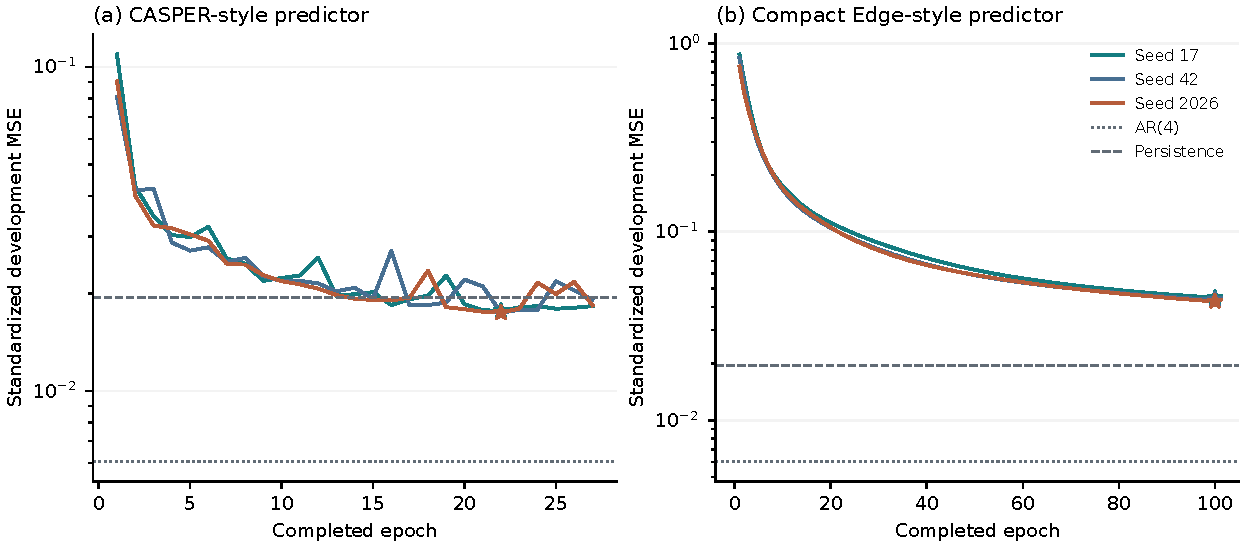
\includegraphics[width=\linewidth]{figures/imu_learning_curves.pdf}
\caption{Normal-development learning curves from the saved training records. Local patience stopping supports greater training adequacy for the CASPER-style architecture; the compact models remain limited by the epoch ceiling. Horizontal control lines refer to the same filtered targets.}\label{fig:imu}
\end{figure}

These results apply to the filtered normal prefix. Median filtering changes the prediction task and introduces dependence, so the autoregressive advantage cannot be assumed to hold for unfiltered attack detection. The patience rule establishes when these runs stopped, not a global optimum, convergence on a representative full dataset or reproduction of the published experiments. This study computes no attack threshold, F1 or recovery score and performs no test-label optimization. Lower normal MSE alone is insufficient evidence of better cyberattack detection.

The run used 764.794 s wall time, 753.252 s CPU, 553.05 MiB sampled peak memory and 2.68 MiB of outputs. Seventeen pre-run synthetic checks and 3,754 fresh-process artifact checks covered checkpoint reloads, score alignment and source identities. The hardware was the same macOS arm64 workstation; process threads and actual budgets are retained in provenance. No neural model was refitted while preparing this manuscript.


\section{Reproducibility, resources and preserved failures}
The local experiment records are E1: \path{recovery_v0.8}; E2: \path{commissioning_v0.9}; E3: \path{casper_convergence_v0.11}; E4: \path{return_bound_v0.12}; and E5: \path{residual_twin_v0.13} followed by \path{attack_audit_v0.14}. Each has source/configuration identities, fitted artifacts where applicable, dependencies, commands, logs, outcomes and verification records. Their split and threshold policies are version-specific and must not be substituted for one another. Later outcome-informed design remains exploratory relative to earlier exposed evidence.

Python 3.12.15 and NumPy 1.26.4 are recorded for the research environment; the IMU fits additionally use TensorFlow 2.16.2. Presentation uses Matplotlib 3.10.0. The workstation is macOS/arm64. The IMU run recorded 18 logical processors; subsequent restricted hardware probes failed and do not supply a verified RAM specification. No GPU result or hardware deployment latency is claimed. The source package records exact interpreter paths and commands without redistributing raw recordings.

E1 consumed 229.20 seconds supervised wall time, 228.07 seconds worker CPU and 167.25 MiB sampled peak memory. E2 consumed 14.75 seconds wall, 14.30 seconds CPU and 113.97 MiB sampled memory. E1's initial launch failed before worker initialization because process monitoring was blocked. E2's first attempt stopped on a reporting-key collision after selection and before fresh generation; a separately recorded repair preserved byte-identical fits and selection. Both failures remain in the experimental record. E5's final audit has no failed run or retry.

The final audit's limits were 120 seconds wall, 90 seconds worker CPU, 1 GiB monitored resident memory and 128 MiB output. Its measured peak from worker \texttt{getrusage} was 99.53 MiB, compared with 90.17 MiB sampled by the supervisor. The shared implementation caches references and scores across variants, so dividing total time by 17 is not a valid per-method benchmark. The manuscript does not infer real-time guarantees from this bounded local run.

The final audit freeze has SHA-256
\begin{center}\small\url{b48a0c3927b465559a8f7b372c2d26ed7148642c97d2435de83995a0ad3be021}.\end{center}
The sealed result package has SHA-256
\begin{center}\small\url{987d8904dda988c7ccd51d61a5e52cf8e162e8f0156286aad89c385813b785dc}.\end{center}
These identities bind provenance, not scientific validity. The revision's asset receipt binds each generated table and figure to saved inputs. Raw observations, vendor manuscripts and private environments are excluded from the editable manuscript archive.

\section{Independent data and published-comparator admission}
\subsection{voraus-AD and MVT-Flow}
The original source is \url{https://media.vorausrobotik.com/voraus-ad-dataset-100hz.parquet}, linked by the author repository \url{https://github.com/vorausrobotik/voraus-ad-dataset}. The file has 1,115,942,833 bytes and SHA-256
\begin{center}\small\url{c90ab1c78af52651b954d41787f7e89d750f0a128b57600b0e5ceec22621f704}.\end{center}
The dataset is CC BY-NC-SA 4.0; the inspected code has a separate MIT license. The primary paper is published in IEEE Transactions on Robotics, volume 40 (2024), pages 438--451, DOI \url{10.1109/TRO.2023.3332224}. Its first arXiv version is dated 8 November 2023.

Metadata-only inspection finds 2,321,690 rows, 137 columns and 2,122 execution identifiers. Labels and settings are constant within each execution. Setting 72 (PRE\_A) supplies all 948 original training executions; the test contains 419 normal and 755 anomalous executions. Per-execution time starts at zero, increases strictly, and has increments from 0.00845194 to 0.01211095 seconds. The largest train and test executions both contain 1,164 rows. These relative times do not establish absolute acquisition order. No process-signal development or test scoring has occurred.

The code revision is
\begin{center}\small\url{a91a86a642d23df58833b792a53de01edfd81abe}.\end{center}
The manuscript describes MVT-Flow, whose code fits the standardizer on normal training data and evaluates a full-execution likelihood. Symmetric temporal convolutions and full-execution scoring make this an offline comparator. Defaults include four coupling blocks, clamp 1.2, width scale two, Adam learning rate $8\times10^{-4}$, batch size 32 and 70 epochs. The test AUROC is computed each epoch, but the inspected code saves the fixed final epoch; this alone does not prove test-based checkpoint selection.

Three discrepancies require explicit treatment. The training loss uses $\|z\|^2-\log|J|$, while the paper and per-sample scoring function use $\tfrac12\|z\|^2-\log|J|$; this changes the relative weighting. The paper describes three convolutions, while the default released block constructs two. A truncation assignment in test padding is overwritten, although the received original release has no test execution longer than the maximum training length, so no effect on that release has been demonstrated. Static inspection and synthetic arithmetic support these observations. They do not establish that the published results used this exact code revision or are invalid.

The source is admitted for a separate real-robot fault/reference study. MVT-Flow is eligible for author-code evaluation under a disclosed protocol, but faithful reproduction remains unresolved until objective, architecture and runtime correspondence are established. Any modified implementation must retain a separate designation. The original test signal values remain unopened. A new partition and feature contract is required before fitting.

\subsection{FactoryNet release boundaries}
The current manuscript is arXiv:2605.09081v5, dated 8 October 2026; its record reports acceptance at AI4Physics and FMSD workshops associated with ICML 2026, not verified main-conference publication. The author data repository is \url{https://huggingface.co/datasets/Forgis/FactoryNet}, inspected at revision \url{3bea3cfc10545d898604f93170108576fd46d518}. Code was inspected at \url{https://github.com/Forgis-Labs/factorynet}, revision \url{651f066d97b704f0824687f1086eeb8f0422a8f3}. No FactoryNet observations were downloaded.

The pinned data card reports 56,591 executions, including 14,847 real and 41,744 simulated. These are author-reported counts, not locally verified observations. The card says its available synthetic snapshot contains the older Isaac Sim 4.5 campaign while the advertised Isaac Sim 5.1 campaign is still uploading. The repository also contains an older description and does not establish a complete mapping to every current-paper experiment. This prevents a blanket claim that the latest full experiment is immediately reproducible.

The corpus includes new recordings and imported voraus-AD, AURSAD and CNC sources. Imported recordings cannot be counted again as independent acquisitions. Context contains fault labels and must not enter a detector indiscriminately. Available signals and missing channels differ by embodiment. Dataset subsets and repository code have distinct licenses. Trusted-command provenance, attack semantics and physical-return annotations are not established by a setpoint field alone. Admission therefore remains partial and no FactoryNet performance is reported.

\clearpage
\section{Covariance-aware return bounds}\label{sec:window}
\subsection{A standard control for current deviation}
Averaging offers a way to reduce noise, but a clearance decision concerns the robot's motion now. The following control accounts for both effects. It separates reference bias from measurement noise instead of treating an empirical residual maximum as a model-error bound. For a dimensionless channel $j$, write
\begin{equation}
 e_{t,j}=v_{t,j}+\beta_{t,j}+\epsilon_{t,j},
 \qquad |\beta_{t,j}|\le B_j,\quad |v_{t,j}-v_{t-1,j}|\le L_j,
 \label{eq:decomposition}
\end{equation}
where $v$ is physical deviation from the nominal response, $\beta$ is reference bias, and $\epsilon$ is measurement noise. Assume a stationary zero-mean Gaussian AR(1) noise process with marginal standard deviation $\sigma_j$ and correlation $0\le\rho_j<1$. The variance of a mean over $m$ consecutive noise observations is
\begin{equation}
 V_{m,j}=\frac{\sigma_j^2}{m^2}
 \left[m+2\sum_{k=1}^{m-1}(m-k)\rho_j^k\right].
 \label{eq:covariance}
\end{equation}
Independence gives $V_{m,j}=\sigma_j^2/m$. Positive serial correlation reduces the effective averaging benefit.

Let $\mathcal M$ contain $K$ fixed windows, let $d$ be the number of channels, and allocate $\alpha_t=6\alpha/(\pi^2t^2)$ using a global clock that does not restart at alarms. Define
\begin{equation}
 U_{t,j}(m)=|\overline e_{t,j}(m)|+B_j
 +\sqrt{2V_{m,j}\log(2dK/\alpha_t)}
 +\frac{L_j(m-1)}{2}.
 \label{eq:windowbound}
\end{equation}
The last term covers motion during the window. Without it, a small average deviation could be mistaken for a small current deviation.

\begin{proposition}
Under the stated Gaussian covariance, bias and increment assumptions, with probability at least $1-\alpha$, $|v_{t,j}|\le U_{t,j}(m)$ simultaneously for every channel, complete registered window and prospective time within a trace. Consequently, the decision
\begin{equation}
 \min_{m\in\mathcal M}U_{t,j}(m)\le\delta_j\qquad(j=1,\ldots,d)
 \label{eq:certificate}
\end{equation}
certifies coordinatewise return on that simultaneous event.
\end{proposition}
\begin{proof}
The Gaussian mean has variance $V_{m,j}$, so its two-sided tail at the square-root term in Equation~\ref{eq:windowbound} is at most $\alpha_t/(dK)$. Sum over channels, registered windows and times, using $\sum_{t=1}^{\infty}\alpha_t=\alpha$. Window overlap and cross-channel dependence do not invalidate this union bound. Finally, $|\overline\beta|\le B_j$ and
$|v_{t,j}-\overline v_{t,j}(m)|\le m^{-1}\sum_{k=0}^{m-1}kL_j=L_j(m-1)/2$.
The triangle inequality gives the result. Each coordinate may use a different minimizing window because all bounds hold simultaneously.
\end{proof}

This control follows from elementary probability bounds and makes no new claim in time-uniform inference. The error allocation is conservative, and the guarantee holds only under the supplied covariance and deterministic bounds. An unknown or invalid observation invalidates the affected windows without restarting the clock. Failure to obtain a certificate leaves return uncertain; it does not generate an attack alarm. Arbitrary colored, heavy-tailed or nonstationary noise is outside the model.

\subsection{Prospective residual experiment}
The diagnostic fixes $d=4$, $\mathcal M=\{1,41,201\}$, $\alpha=0.05$, $\delta_j=0.1$ and $B_j=0.01$. Four $(\sigma,\rho)$ settings are $(0.03,0)$, $(0.06,0)$, $(0.03,0.8)$ and $(0.06,0.95)$, with channel standard-deviation multipliers $(1,0.8,1.1,0.9)$. For phases $\phi_j=(0,0.4,0.8,1.2)$, bias is $0.01\cos(0.003t+\phi_j)$. The physical-deviation signals are zero, $0.02\sin(0.004t+\phi_j)$, and $0.02\sin(0.04t+\phi_j)$, termed settled, slow and faster variation. They always lie within tolerance. The corresponding increment bound is $L_j=2a|\sin(\omega/2)|$, derived from the declared amplitude and frequency.

Each trace contains 1,200 samples, with the first noise value drawn from the stationary marginal. Seeds 17,42,2026 produce three independent innovation arrays reused across settings, giving 36 paired constructed traces rather than 36 independent acquisitions. The common reporting support is samples 201--1,200, or 1,000 endpoints per trace. The error statement is marginal per trace; no simultaneous 95\% guarantee across this whole matrix is claimed.

All four valid controls---the three fixed windows and their simultaneous envelope---receive identical residuals and parameter bounds. Two deliberately misspecified controls set $\rho=0$ for the 41- and 201-sample windows. Every variant and all 216 outcomes are retained. The criterion requires at least 95\% of common endpoints certified on every trace by the envelope. Parameters and conditions were recorded before generating outcomes; none was changed afterward.

The generator constructs these residual signals directly; it does not run the robot dynamics of Section~\ref{sec:simulation}. It also supplies the noise, bias and increment bounds. This lets the experiment isolate their mathematical effects, but leaves open how an operational monitor would obtain those bounds from commissioning data. The diagnostic contains no attacks, threshold fitting or model learning, and measures no post-attack recovery delay.

\subsection{Results and implications}
The envelope passes on 20 of 36 traces and therefore fails the overall normal-feasibility requirement. Table~\ref{tab:window} includes every condition group and its range across seeds; Figure~\ref{fig:window} shows the lowest fraction in each group. The instantaneous control certifies no endpoints. Averaging helps in several settings, but taking the longest window or assuming independent noise does not work uniformly.

\begin{table}[htbp]\centering\small
\caption{Residual diagnostic: simultaneous-envelope certificates on normal synthetic residuals. Each range spans the three seeds, each with 1,000 common endpoints. Passing requires at least 95\% on each trace.}\label{tab:window}
\setlength{\tabcolsep}{5pt}
\begin{tabular}{llrr}\toprule
Noise setting & Deviation profile & Certificates (\%) & Passes \\\midrule
Independent, low & Settled & 100.0--100.0 & 3/3 \\
Independent, low & Slow variation & 100.0--100.0 & 3/3 \\
Independent, low & Faster variation & 100.0--100.0 & 3/3 \\
Independent, high & Settled & 100.0--100.0 & 3/3 \\
Independent, high & Slow variation & 100.0--100.0 & 3/3 \\
Independent, high & Faster variation & 17.2--25.6 & 0/3 \\
Correlated, low & Settled & 100.0--100.0 & 3/3 \\
Correlated, low & Slow variation & 85.8--100.0 & 2/3 \\
Correlated, low & Faster variation & 0.0--0.0 & 0/3 \\
Correlated, high & Settled & 0.0--0.0 & 0/3 \\
Correlated, high & Slow variation & 0.0--0.0 & 0/3 \\
Correlated, high & Faster variation & 0.0--0.0 & 0/3 \\
\bottomrule\end{tabular}

\end{table}

\begin{figure}[htbp]\centering
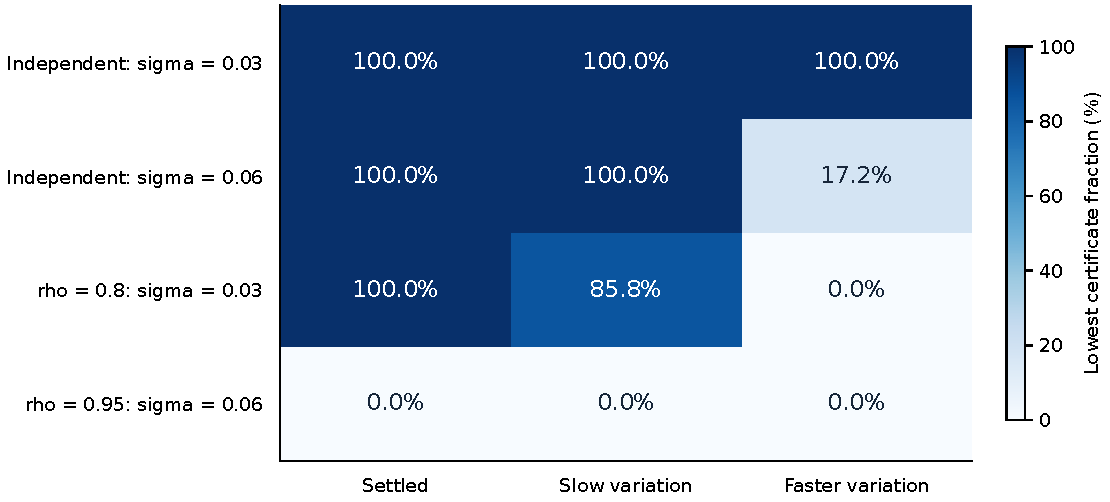
\includegraphics[width=0.88\linewidth]{figures/window_feasibility.pdf}
\caption{Lowest certificate fraction across seeds for each synthetic residual condition. All physical-deviation signals are within tolerance. A certificate establishes only the conditional bound in Equation~\ref{eq:certificate}; low coverage is not an attack-detection result.}\label{fig:window}
\end{figure}

For independent low noise with faster variation, window 41 certifies every endpoint, whereas window 201 certifies none. The longer window's drift allowance consumes its noise benefit. Under correlated low noise and slow variation, the envelope's fractions are 100\%, 85.8\% and 100\%: their 95.27\% average does not satisfy the all-traces criterion. At $\rho=0.95$ and $\sigma=0.06$, no valid control certifies any common endpoint, even for the settled profile. The misspecified 201-sample control would certify 91.53\% on average for that settled profile, but its uncertainty claim no longer follows from the actual covariance.

There are no observed coverage violations, but all the constructed deviations lie within tolerance. These traces cannot estimate rare unsafe-clearing risk or establish performance near the tolerance boundary. The experiment instead exposes the competing effects of window length: more averaging reduces noise uncertainty while increasing the allowance for current-state variation. Choosing a window after seeing its outcome would not resolve that conflict. The decision needs defensible information about noise and motion.

The diagnostic completed in 0.565 s wall time and 0.459 s CPU time, with 39.81 MiB sampled peak memory and 11.07 MiB of outputs. Twenty synthetic software checks and 2,665 saved-artifact checks support its implementation. These costs cover the entire small diagnostic and cannot be interpreted as robot deployment latency.

\end{document}
